\newpage
\section{Objetivos}
\label{sc:objetivos_}


{
Para apresentar uma nova forma de solução dos problemas enfrentados pelos fazendeiros, o objetivo é integrar múltiplas tecnologias, se apropriando do uso do IoT em conjunto com outros sistemas, tais como RSSI, Wi-Fi, Bluetooth Low Energy, criando um conjunto que possibilite ao fazendeiro gerenciar e localizar seu gado.
}

{
Esse sistema seria composto por antenas fixas espalhadas na área a ser monitorada e pela placa de transmissão acoplada na etiqueta de cada animal. No momento em que a placa acoplada transmite sinal para as antenas, o sinal seria processado e então serial calculada a sua localização aproximada por meio da trilateração, e esses dados ficariam dispostos ao agricultor.
}

{
A figura \ref{fig:modelo_simplificado_projeto} esboça de forma simplificada o sistema de transmissão de dados entre uma vaca com a placa desenvolvida acoplada em sua etiqueta de identificação entre duas antenas fixas. A partir dos cálculos realizados o fazendeiro poderá saber a localização aproximada da vaca em sua fazenda.
}

\begin{figure}[htp]
    \centering
    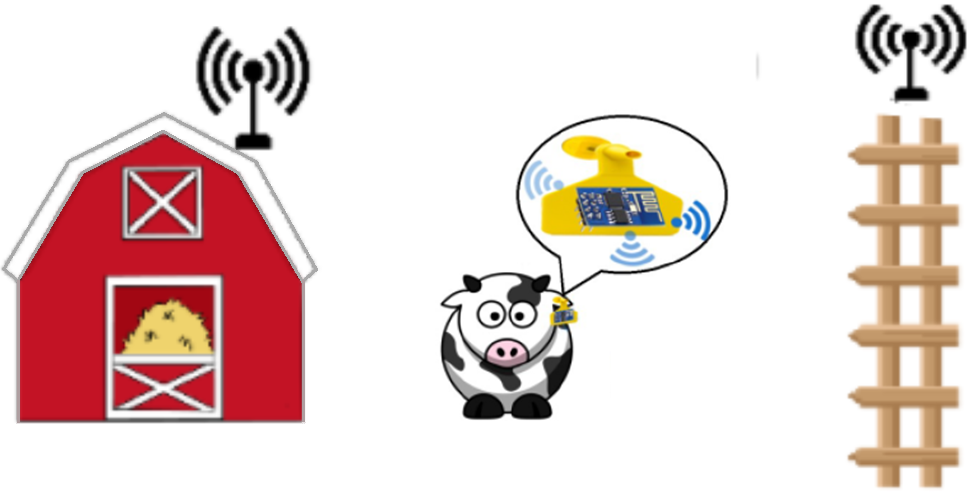
\includegraphics[scale = 0.5]{img/Resumo_projeto.png}
    \caption{Modelo simplificado projeto}
    \label{fig:modelo_simplificado_projeto}
\end{figure}


